\begin{figure}[h]
    \centering
    \label{fig:dnn-example}
    
    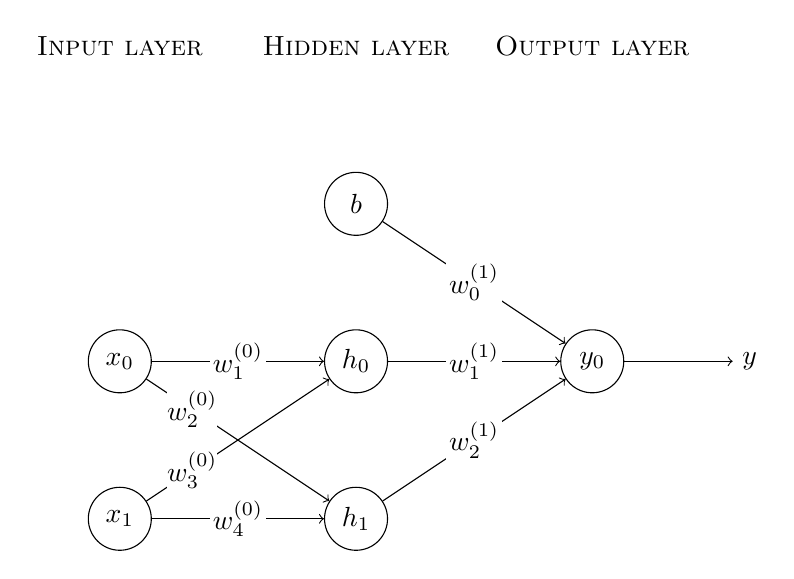
\begin{tikzpicture}
        \def\vert{2}
        \def\hori{3}
        \tikzstyle{place}=[circle, draw=black, minimum size=8mm]
        \tikzstyle{label}=[inner sep=1pt, fill=white]
        
        % Input
        \draw node at (0 * \hori, 4 * \vert) [black, ] {\textsc{Input layer}};
        
        \draw node at (0 * \hori, 2 * \vert) [place] (input_0) {$x_0$};	
        \draw node at (0 * \hori, 1 * \vert) [place] (input_1) {$x_1$};
        
        
        % Hidden
        \draw node at (1 * \hori, 4 * \vert) [black, ] {\textsc{Hidden layer}};
        
        \draw node at (1 * \hori, 3 * \vert) [place] (hidden_0) {$b$};
        \draw node at (1 * \hori, 2 * \vert) [place] (hidden_1) {$h_0$};	
        \draw node at (1 * \hori, 1 * \vert) [place] (hidden_2) {$h_1$};	
        
        % Output
        \draw node at (2 * \hori, 4 * \vert) [black, ] {\textsc{Output layer}};
        
        \draw node at (2 * \hori, 2 * \vert) [place] (output_0) {$y_0$};
        
        % Out
        \node at (8, 2 * \vert) [black, ] (out_0) {$y$};
		
        % Input -> Hidden
        % \foreach \i in {0,...,1}
        %  	 \foreach \j in {1,...,2}
        %		 \draw [->] (input_\i) to node[near start, below] {$w_{\i}^{(0)}$} (hidden_\j);
        \draw [->] (input_0) to node[label] {$w_{1}^{(0)}$} (hidden_1);
        \draw [->] (input_0) to node[label, near start, inner sep=0pt] {$w_{2}^{(0)}$} (hidden_2);
        \draw [->] (input_1) to node[label, near start, inner sep=0pt] {$w_{3}^{(0)}$} (hidden_1);
        \draw [->] (input_1) to node[label] {$w_{4}^{(0)}$} (hidden_2);
        
        
        % Hidden -> Output
        \foreach \i in {0,...,2}
		\foreach \j in {0,...,0}
        \draw [->] (hidden_\i) to node[label] {$w_{\i}^{(1)}$} (output_\j);
        
        \foreach \i in {0,...,0}
		\draw [->] (output_\i) to (out_\i);
        
    \end{tikzpicture}
    \caption{Example DNN with a single hidden layer}
\end{figure}